\documentclass[border=12pt]{standalone}
\usepackage[dvipsnames]{xcolor}
\usepackage{amsmath}
\usepackage{tikz}
\usetikzlibrary{arrows.meta,positioning,fit,backgrounds,calc}

% ---------------- colours (matching protograph_construction.tex) ----------------
\definecolor{schemagreen}{RGB}{198,239,206}  % instance / output (green)
\definecolor{ransub}{RGB}{197,233,243}        % relation (cyan)
\definecolor{agentfill}{RGB}{231,222,242}     % class (lavender)
\definecolor{midfill}{RGB}{218,232,247}       % bound / term (blue)
\definecolor{leaffill}{RGB}{244,248,253}      % neighbour / processing (pale blue)
\definecolor{hdr}{RGB}{225,225,225}           % sum node (gray)
\definecolor{darknavy}{RGB}{18,32,86}         % class edges / labels (dark navy)

\newcommand{\ttag}[1]{{\scriptsize\bfseries\textcolor{darknavy}{#1}}}

\begin{document}
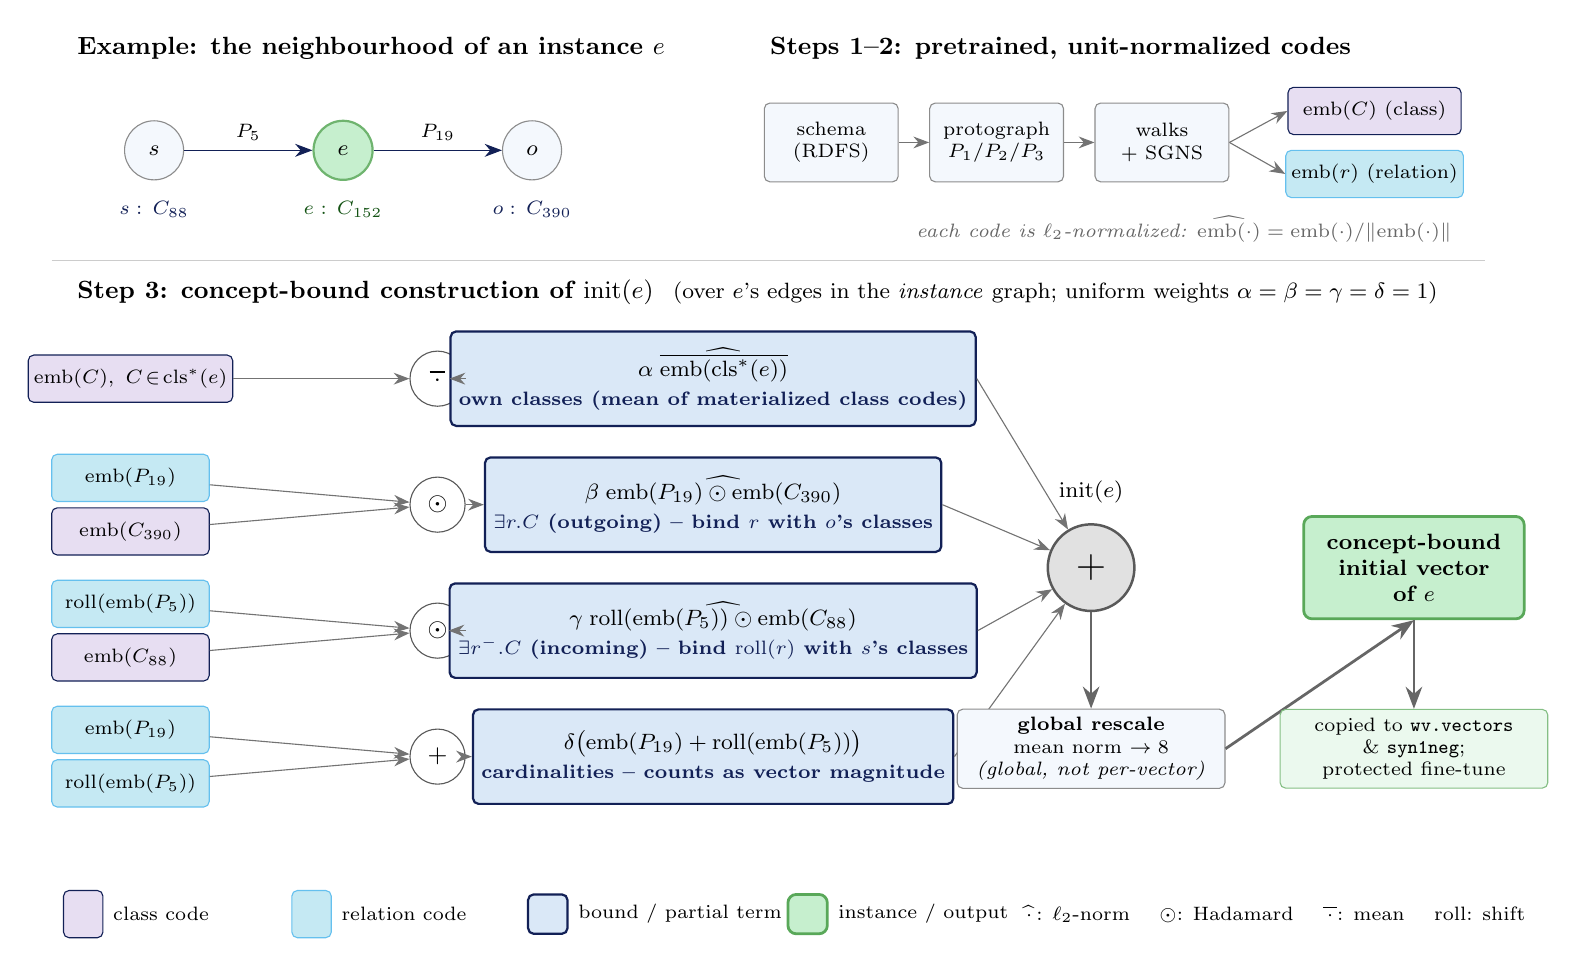
\begin{tikzpicture}[
  font=\footnotesize,
  inst/.style={circle, draw=ForestGreen!65, line width=0.8pt, fill=schemagreen,
               minimum size=7.5mm, font=\footnotesize\bfseries},
  nbr/.style={circle, draw=black!45, fill=leaffill, minimum size=7.5mm, font=\footnotesize},
  ccode/.style={rounded corners=2pt, draw=darknavy, fill=agentfill,
                minimum height=6mm, minimum width=20mm, inner sep=2pt, font=\scriptsize},
  rcode/.style={rounded corners=2pt, draw=Cerulean!65, fill=ransub,
                minimum height=6mm, minimum width=20mm, inner sep=2pt, font=\scriptsize},
  op/.style={circle, draw=black!65, fill=white, minimum size=7mm, font=\small},
  part/.style={rounded corners=2pt, draw=darknavy, line width=0.8pt, fill=midfill,
               minimum height=12mm, minimum width=52mm, inner sep=3pt, align=center, font=\footnotesize},
  proc/.style={rounded corners=2pt, draw=black!45, fill=leaffill,
               minimum height=10mm, minimum width=30mm, inner sep=3pt, align=center, font=\scriptsize},
  final/.style={rounded corners=3pt, draw=ForestGreen!75, line width=1pt, fill=schemagreen,
                minimum height=13mm, minimum width=28mm, inner sep=3pt, align=center, font=\footnotesize\bfseries},
  sumn/.style={circle, draw=black!65, line width=0.9pt, fill=hdr, minimum size=11mm, font=\Large},
  arr/.style={-{Stealth[length=2mm]}, draw=black!55},
  flow/.style={-{Stealth[length=2.8mm]}, draw=black!60, line width=1pt},
  hdrf/.style={font=\small\bfseries},
  edge/.style={-{Stealth[length=2.2mm]}, draw=darknavy},
]

% ============================================================
% TOP-LEFT: example neighbourhood of instance e
% ============================================================
\node[hdrf, anchor=west] at (-0.4,9.6) {Example: the neighbourhood of an instance $e$};
\node[nbr]  (s) at (0.7,8.3) {$s$};
\node[inst] (e) at (3.1,8.3) {$e$};
\node[nbr]  (o) at (5.5,8.3) {$o$};
\draw[edge] (s) -- (e) node[midway, above, font=\scriptsize] {$P_{5}$};
\draw[edge] (e) -- (o) node[midway, above, font=\scriptsize] {$P_{19}$};
\node[font=\scriptsize, text=darknavy]      at (0.7,7.55) {$s:\,C_{88}$};
\node[font=\scriptsize, text=ForestGreen!60!black]  at (3.1,7.55) {$e:\,C_{152}$};
\node[font=\scriptsize, text=darknavy]      at (5.5,7.55) {$o:\,C_{390}$};

% ============================================================
% TOP-RIGHT: where the codes come from (Steps 1-2)
% ============================================================
\node[hdrf, anchor=west] at (8.4,9.6) {Steps 1--2: pretrained, unit-normalized codes};
\node[proc, minimum width=17mm] (sc)  at (9.3,8.4) {schema\\(RDFS)};
\node[proc, minimum width=17mm] (pg)  at (11.4,8.4) {protograph\\$P_1/P_2/P_3$};
\node[proc, minimum width=17mm] (sg)  at (13.5,8.4) {walks\\$+$ SGNS};
\node[ccode, minimum width=22mm] (cb) at (16.2,8.8) {$\mathrm{emb}(C)$ \scriptsize(class)};
\node[rcode, minimum width=22mm] (rb) at (16.2,8.0) {$\mathrm{emb}(r)$ \scriptsize(relation)};
\draw[arr] (sc) -- (pg);
\draw[arr] (pg) -- (sg);
\draw[arr] (sg.east) -- (cb.west);
\draw[arr] (sg.east) -- (rb.west);
\node[font=\scriptsize\itshape, text=black!60, anchor=east] at (17.3,7.3)
  {each code is $\ell_2$-normalized: $\widehat{\mathrm{emb}(\cdot)}=\mathrm{emb}(\cdot)/\lVert\mathrm{emb}(\cdot)\rVert$};

% separating rule
\draw[black!20] (-0.6,6.9) -- (17.6,6.9);
\node[hdrf, anchor=west] at (-0.4,6.5)
  {Step 3: concept-bound construction of $\mathrm{init}(e)$ \ \footnotesize\mdseries (over $e$'s edges in the \emph{instance} graph; uniform weights $\alpha=\beta=\gamma=\delta=1$)};

% ============================================================
% MIDDLE: the four terms (one row each)
% ============================================================
\def\ya{5.4}\def\yb{3.8}\def\yc{2.2}\def\yd{0.6}
\def\xin{0.4}\def\xop{4.3}\def\xpart{7.8}

% ---- alpha : own classes ----
\node[ccode] (ca) at (\xin,\ya) {$\mathrm{emb}(C),\ C\!\in\!\mathrm{cls}^*(e)$};
\node[op]    (oa) at (\xop,\ya) {$\overline{\,\cdot\,}$};
\node[part]  (pa) at (\xpart,\ya)
  {$\alpha\;\widehat{\overline{\mathrm{emb}(\mathrm{cls}^*(e))}}$\\[1pt] \ttag{own classes (mean of materialized class codes)}};
\draw[arr] (ca) -- (oa);
\draw[arr] (oa) -- (pa);

% ---- beta : outgoing exists r.C ----
\node[rcode] (rb1) at (\xin,\yb+0.34) {$\mathrm{emb}(P_{19})$};
\node[ccode] (cb1) at (\xin,\yb-0.34) {$\mathrm{emb}(C_{390})$};
\node[op]    (ob)  at (\xop,\yb) {$\odot$};
\node[part]  (pb)  at (\xpart,\yb)
  {$\beta\;\widehat{\mathrm{emb}(P_{19})\odot \mathrm{emb}(C_{390})}$\\[1pt] \ttag{$\exists r.C$ (outgoing) -- bind $r$ with $o$'s classes}};
\draw[arr] (rb1) -- (ob);
\draw[arr] (cb1) -- (ob);
\draw[arr] (ob) -- (pb);

% ---- gamma : incoming exists r^-.C ----
\node[rcode] (rc1) at (\xin,\yc+0.34) {$\mathrm{roll}(\mathrm{emb}(P_{5}))$};
\node[ccode] (cc1) at (\xin,\yc-0.34) {$\mathrm{emb}(C_{88})$};
\node[op]    (oc)  at (\xop,\yc) {$\odot$};
\node[part]  (pc)  at (\xpart,\yc)
  {$\gamma\;\widehat{\mathrm{roll}(\mathrm{emb}(P_{5}))\odot \mathrm{emb}(C_{88})}$\\[1pt] \ttag{$\exists r^{-}.C$ (incoming) -- bind $\mathrm{roll}(r)$ with $s$'s classes}};
\draw[arr] (rc1) -- (oc);
\draw[arr] (cc1) -- (oc);
\draw[arr] (oc) -- (pc);

% ---- delta : relation counts ----
\node[rcode] (rd1) at (\xin,\yd+0.34) {$\mathrm{emb}(P_{19})$};
\node[rcode] (rd2) at (\xin,\yd-0.34) {$\mathrm{roll}(\mathrm{emb}(P_{5}))$};
\node[op]    (od)  at (\xop,\yd) {$+$};
\node[part]  (pd)  at (\xpart,\yd)
  {$\delta\big(\mathrm{emb}(P_{19})+\mathrm{roll}(\mathrm{emb}(P_{5}))\big)$\\[1pt] \ttag{cardinalities -- counts as vector magnitude}};
\draw[arr] (rd1) -- (od);
\draw[arr] (rd2) -- (od);
\draw[arr] (od) -- (pd);

% ============================================================
% RIGHT: sum -> global rescale -> final vector -> matrices
% ============================================================
\def\xsum{12.6}
\node[sumn] (sum) at (\xsum,3.0) {$+$};
\node[font=\footnotesize, anchor=south] at (\xsum,3.7) {$\mathrm{init}(e)$};
\draw[arr] (pa.east) -- (sum);
\draw[arr] (pb.east) -- (sum);
\draw[arr] (pc.east) -- (sum);
\draw[arr] (pd.east) -- (sum);

\node[proc, minimum width=34mm] (resc) at (\xsum,0.7)
  {\textbf{global rescale}\\ mean norm $\to 8$\\ \emph{(global, not per-vector)}};
\draw[flow] (sum) -- (resc);

\node[final] (fin) at (16.7,3.0) {concept-bound\\ initial vector\\ of $e$};
\draw[flow] (resc.east) -- (fin.south);

\node[proc, minimum width=34mm, draw=ForestGreen!55, fill=schemagreen!35] (write) at (16.7,0.7)
  {copied to \texttt{wv.vectors}\\ \& \texttt{syn1neg};\\ protected fine-tune};
\draw[flow] (fin) -- (write);

% ============================================================
% LEGEND
% ============================================================
\node[ccode, minimum width=5mm] (l1) at (-0.2,-1.4) {};
\node[anchor=west, font=\scriptsize] at (l1.east) {class code};
\node[rcode, minimum width=5mm] (l2) at (2.7,-1.4) {};
\node[anchor=west, font=\scriptsize] at (l2.east) {relation code};
\node[part, minimum width=5mm, minimum height=5mm] (l3) at (5.7,-1.4) {};
\node[anchor=west, font=\scriptsize] at (l3.east) {bound / partial term};
\node[final, minimum width=5mm, minimum height=5mm] (l4) at (9.0,-1.4) {};
\node[anchor=west, font=\scriptsize] at (l4.east) {instance / output};
\node[anchor=west, font=\scriptsize] at (11.6,-1.4)
  {$\widehat{\,\cdot\,}$: $\ell_2$-norm \quad $\odot$: Hadamard \quad $\overline{\,\cdot\,}$: mean \quad $\mathrm{roll}$: shift};

\end{tikzpicture}
\end{document}
